\documentclass[tikz,border=6pt]{standalone}
\begin{document}
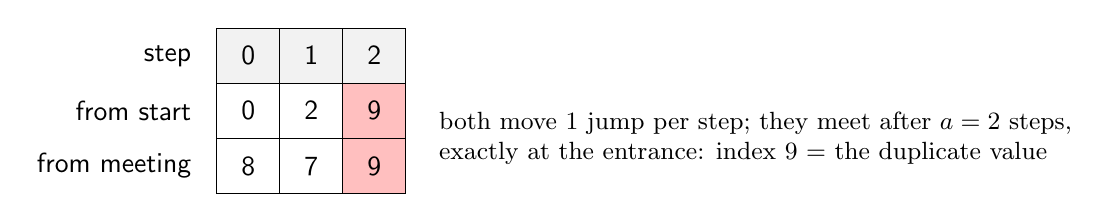
\begin{tikzpicture}[font=\sffamily,cell/.style={draw,minimum width=8mm,minimum height=7mm}]
\node[anchor=east] at (-0.6,0) {step};
\node[anchor=east] at (-0.6,-0.7) {from start};
\node[anchor=east] at (-0.6,-1.4) {from meeting};
\foreach \a/\b [count=\t from 0] in {0/8,2/7,9/9} { \node[cell,fill=gray!10] at (\t*0.8,0) {\t}; \node[cell] at (\t*0.8,-0.7) {\a}; \node[cell] at (\t*0.8,-1.4) {\b}; }
\node[cell,fill=red!25] at (1.6,-0.7) {9}; \node[cell,fill=red!25] at (1.6,-1.4) {9};
\node[anchor=west,font=\small,align=left] at (2.3,-1.05) {both move 1 jump per step; they meet after $a=2$ steps,\\exactly at the entrance: index 9 = the duplicate value};
\end{tikzpicture}
\end{document}
